\documentclass[12pt,a4paper]{article}

% --- Page Layout -------------------------------------------------------------
\usepackage[a4paper, margin=0.8in, headheight=14pt]{geometry}

% --- Fonts (XeLaTeX) ---------------------------------------------------------
\usepackage{fontspec}
\usepackage{unicode-math}
\setmainfont{TeX Gyre Pagella}
\setmonofont[Scale=0.88]{TeX Gyre Cursor}
\setmathfont{Latin Modern Math}

% --- Packages ---------------------------------------------------------------
\usepackage{xcolor}
\usepackage{titlesec}
\usepackage{enumitem}
\usepackage{tabularx}
\usepackage{booktabs}
\usepackage{array}
\usepackage{amsmath}
\usepackage{tikz}
\usetikzlibrary{shapes.geometric, arrows.meta, positioning, calc, fit, decorations.pathreplacing}
\usepackage{tcolorbox}
\tcbuselibrary{skins, breakable}
\usepackage{hyperref}
\usepackage{fancyhdr}
\usepackage{graphicx}
\usepackage{microtype}
\hyphenpenalty=10000
\exhyphenpenalty=10000
\sloppy
\usepackage{caption}
\usepackage{setspace}
\usepackage{multirow}
\usepackage{tocloft}

% --- Q&A helper --------------------------------------------------------------
\newcommand{\Q}[1]{\textbf{#1}\par\noindent\ignorespaces}

% --- Colour Palette ----------------------------------------------------------
\definecolor{myred}{RGB}{196,30,58}
\definecolor{mydark}{RGB}{30,30,50}
\definecolor{mygreen}{RGB}{14,120,80}
\definecolor{myteal}{RGB}{0,130,140}
\definecolor{myamber}{RGB}{180,100,0}
\definecolor{mypurple}{RGB}{100,30,160}
\definecolor{mygray}{RGB}{246,247,249}
\definecolor{mgframe}{RGB}{180,185,200}
\definecolor{watermark}{RGB}{145,150,170}
\definecolor{hdrred}{RGB}{250,232,235}
\definecolor{hdrgreen}{RGB}{220,244,233}
\definecolor{hdrteal}{RGB}{220,242,244}
\definecolor{hdramber}{RGB}{253,242,215}
\definecolor{hdrpurple}{RGB}{238,228,255}

% --- Section Formatting ------------------------------------------------------
\titleformat{\section}
  {\large\bfseries\color{myred}}{\thesection.}{0.5em}{}
  [\vspace{1pt}{\color{myred}\rule{\linewidth}{0.8pt}}]
\titleformat{\subsection}
  {\normalsize\bfseries\color{myteal}}{\thesubsection}{0.5em}{}
\titlespacing*{\section}{0pt}{18pt}{7pt}
\titlespacing*{\subsection}{0pt}{11pt}{4pt}

% --- Paragraph ---------------------------------------------------------------
\setlength{\parindent}{0pt}
\setlength{\parskip}{4pt}

% --- TOC Styling -------------------------------------------------------------
\renewcommand{\cfttoctitlefont}{\large\bfseries\color{myred}}
\renewcommand{\cftaftertoctitle}{\par\noindent{\color{myred}\rule{\linewidth}{0.8pt}}}
\setlength{\cftbeforetoctitleskip}{0pt}
\setlength{\cftaftertoctitleskip}{6pt}
\renewcommand{\cftsecfont}{\normalsize\bfseries\color{mydark}}
\renewcommand{\cftsecpagefont}{\normalsize\bfseries\color{mydark}}
\renewcommand{\cftsecleader}{\cftdotfill{\cftdotsep}}
\setlength{\cftbeforesecskip}{7pt}
\renewcommand{\cftsubsecfont}{\small\color{mydark}}
\renewcommand{\cftsubsecpagefont}{\small\color{mydark}}
\setlength{\cftbeforesubsecskip}{3pt}
\setlength{\cftsubsecindent}{1.4em}

% --- Table helpers -----------------------------------------------------------
\renewcommand{\arraystretch}{1.45}
\setlength{\tabcolsep}{6pt}
\newcolumntype{B}[1]{>{\small\bfseries\raggedright\arraybackslash}m{#1}}
\newcolumntype{Y}{>{\small\raggedright\arraybackslash}X}
\renewcommand{\tabularxcolumn}[1]{m{#1}}

% --- Header / Footer ---------------------------------------------------------
\pagestyle{fancy}
\fancyhf{}
\fancyhead[L]{\small\color{myred}\textbf{BS-PH101}\;\color{mydark}--- Physics-I}
\fancyhead[R]{\small\color{myteal}\textbf{Module 5 Notes}}
\fancyfoot[C]{\small\color{mydark}\thepage}
\fancyfoot[R]{\small\color{watermark}\textit{\copyright\ Biraj}}
\renewcommand{\headrulewidth}{0.5pt}
\renewcommand{\footrulewidth}{0.3pt}

% --- Hyperref ---------------------------------------------------------------
\hypersetup{
  colorlinks=true, linkcolor=myteal, urlcolor=myteal,
  pdfauthor={Biraj Sarkar},
  pdftitle={BS-PH101 --- Module 5 Notes}
}

% --- tcolorbox styles --------------------------------------------------------
\tcbset{
  tikzbox/.style={
    colback=mygray, colframe=mgframe, boxrule=0.6pt, arc=4pt,
    left=8pt, right=8pt, top=6pt, bottom=6pt,
    colbacktitle=mgframe, coltitle=mydark, fonttitle=\small\bfseries
  },
  defbox/.style={
    colback=hdrgreen, colframe=mygreen, boxrule=0.8pt, arc=4pt,
    left=9pt, right=9pt, top=6pt, bottom=6pt,
    colbacktitle=mygreen, coltitle=white, fonttitle=\small\bfseries
  },
  formulabox/.style={
    colback=hdrteal, colframe=myteal, boxrule=0.8pt, arc=4pt,
    left=9pt, right=9pt, top=7pt, bottom=7pt,
    colbacktitle=myteal, coltitle=white, fonttitle=\small\bfseries
  },
  examplebox/.style={
    colback=hdramber, colframe=myamber, boxrule=0.8pt, arc=4pt,
    left=9pt, right=9pt, top=6pt, bottom=6pt,
    colbacktitle=myamber, coltitle=white, fonttitle=\small\bfseries
  },
  masonbox/.style={
    colback=hdrpurple, colframe=mypurple, boxrule=0.8pt, arc=4pt,
    left=9pt, right=9pt, top=6pt, bottom=6pt,
    colbacktitle=mypurple, coltitle=white, fonttitle=\small\bfseries
  },
  exambox/.style={
    colback=hdrpurple, colframe=mypurple, boxrule=1pt, arc=5pt,
    left=10pt, right=10pt, top=8pt, bottom=8pt,
    colbacktitle=mypurple, coltitle=white, fonttitle=\bfseries,
    breakable, title after break={\textbf{Frequently Asked / Viva Questions (contd.)}}
  }
}
\tcbset{breakable}

% --- TikZ Styles -------------------------------------------------------------
\tikzset{
  block/.style={rectangle, draw=myteal, fill=hdrteal, text width=2.4cm, align=center, minimum height=0.95cm, font=\small, rounded corners=3pt, line width=0.7pt},
  redblock/.style={rectangle, draw=myred, fill=hdrred, text width=2.4cm, align=center, minimum height=0.95cm, font=\small, rounded corners=3pt, line width=0.7pt},
  arrow/.style={-Stealth, thick, color=mydark},
  redarrow/.style={-Stealth, thick, color=myred},
  line/.style={thick, color=mydark}
}

\begin{document}

% --- Title Page --------------------------------------------------------------
\begin{center}
  {\LARGE\bfseries\color{myred} BS-PH101 --- Physics-I}\\[5pt]
  {\normalsize\color{mydark} Semester I/II \quad$\bullet$\quad 3L:1T:0P \quad$\bullet$\quad 4 Credits}\\[3pt]
  {\normalsize\color{myteal}\textbf{Module 5 Comprehensive Exam Notes: Statistical Mechanics}}\\[3pt]
  {\small\color{mydark} CGEC \;$|$\; B.Tech ECE (2023--27) \;$|$\; \textit{Biraj Sarkar}}
\end{center}
\vspace{2pt}
\noindent{\color{myred}\rule{\linewidth}{1.5pt}}
\vspace{2pt}
\hypersetup{linkcolor=mydark}
\tableofcontents
\hypersetup{linkcolor=myteal}
\newpage

% =============================================================================
% SECTION 1: MACROSTATE, MICROSTATE & PHASE SPACE
% =============================================================================
\section{Macrostate, Microstate, Phase Space, and Ensembles}

\subsection{Basic Concepts of Statistical Mechanics}

Statistical mechanics connects the microscopic behavior of individual atoms/molecules with the macroscopic thermodynamic properties ($P, V, T, S$) of a system.

\begin{tcolorbox}[defbox, title={\textbf{Definitions: Macrostate, Microstate, and Phase Space}}]
\begin{itemize}[leftmargin=*, itemsep=2pt]
  \item \textbf{Macrostate:} The macroscopic state of a system specified by overall thermodynamic variables (e.g. $(N, V, E)$ or $(N, V, T)$).
  \item \textbf{Microstate:} A specific detailed configuration of the system specifying the exact position ($\vec{r}_i$) and momentum ($\vec{p}_i$) of every individual particle.
  \item \textbf{Phase Space:} A $6N$-dimensional conceptual space formed by 3 position coordinates $(x,y,z)$ and 3 momentum coordinates $(p_x,p_y,p_z)$ for each of $N$ particles. The elementary phase cell volume in quantum mechanics is $h^3$.
  \item \textbf{Thermodynamic Probability ($W$):} The total number of microstates corresponding to a given macrostate.
\end{itemize}
\end{tcolorbox}

\begin{tcolorbox}[formulabox, title={\textbf{Boltzmann Entropy Relation}}]
\begin{equation}
S = k_B \ln W
\end{equation}
where $k_B = 1.38 \times 10^{-23}\text{ J/K}$ is Boltzmann's constant, and $W$ is the thermodynamic probability.
\end{tcolorbox}

\subsection{Statistical Ensembles}

An \textbf{ensemble} is a large collection of independent, macroscopically identical systems existing in different microstates.

\textbf{Three Main Gibbs Ensembles:}\par\vspace{6pt}\noindent
\begin{tabularx}{\linewidth}{|B{3.2cm}|Y|Y|}
\hline
\textbf{Ensemble} & \textbf{Fixed Parameters} & \textbf{Physical System Example} \\
\hline
\textbf{Microcanonical} & Number $N$, Volume $V$, Energy $E$ (Rigid, isolated, insulated walls). & Isolated system with zero heat exchange. \\
\hline
\textbf{Canonical} & Number $N$, Volume $V$, Temperature $T$ (Diathermal walls in heat bath). & Closed system exchanging heat with a reservoir. \\
\hline
\textbf{Grand Canonical} & Chem. potential $\mu$, Volume $V$, Temp. $T$ (Permeable, diathermal walls). & Open system exchanging both energy and particles. \\
\hline
\end{tabularx}

\begin{tcolorbox}[examplebox, title={\textbf{Solved Problem 1: Microstates and Entropy}}]
\textbf{Problem:} Calculate the number of microstates and thermodynamic probability $W$ for distributing $N = 4$ distinguishable particles in 2 equal compartments. Find the entropy of the most probable state.

\textbf{Solution:}\par\noindent
\begin{enumerate}[leftmargin=*, itemsep=2pt]
  \item Total number of microstates = $2^N = 2^4 = \mathbf{16}$.
  \item Macrostates are given by $(n_1, n_2)$ where $n_1 + n_2 = 4$:
  \begin{itemize}[leftmargin=*, itemsep=1pt]
    \item $(4,0): W = \frac{4!}{4!0!} = 1$
    \item $(3,1): W = \frac{4!}{3!1!} = 4$
    \item $(2,2): W = \frac{4!}{2!2!} = \mathbf{6} \quad (\text{Most Probable Macrostate})$
    \item $(1,3): W = 4$
    \item $(0,4): W = 1$
  \end{itemize}
  \item Entropy of most probable macrostate $(2,2)$:
   \begin{equation}
   S = k_B \ln(6) = (1.38 \times 10^{-23}) \times 1.7917 = \mathbf{2.47 \times 10^{-23}\text{ J/K}}
   \end{equation}
\end{enumerate}
\end{tcolorbox}

% =============================================================================
% SECTION 2: DENSITY OF STATES
% =============================================================================
\section{Density of States}

\subsection{Derivation of Density of States in 3D}

The \textbf{Density of States ($g(E)dE$)} represents the number of available quantum states per unit volume in the energy range between $E$ and $E + dE$.

\begin{tcolorbox}[formulabox, title={\textbf{3D Free Particle Density of States Derivation}}]
In momentum space, momentum $p = \sqrt{2mE}$. The volume of momentum sphere of radius $p$ is $V_p = \frac{4}{3}\pi p^3 = \frac{4}{3}\pi (2mE)^{3/2}$.
The number of spatial-momentum phase cells of volume $h^3$ inside spatial volume $V$ is:
\begin{equation}
N(E) = \frac{V \cdot \frac{4}{3}\pi (2mE)^{3/2}}{h^3} = \frac{4\pi V (2m)^{3/2}}{3 h^3} E^{3/2}
\end{equation}
Taking the derivative with respect to $E$ gives $g(E) = \frac{dN(E)}{dE}$:
\begin{equation}
g(E) dE = \frac{4\pi V (2m)^{3/2}}{h^3} E^{1/2} dE
\end{equation}
Including electron spin degeneracy $g_s = 2s+1 = 2$ for electrons:
\begin{equation}
g_e(E) dE = \frac{8\pi V (2m)^{3/2}}{h^3} E^{1/2} dE
\end{equation}
\end{tcolorbox}

\textbf{Density of States in Lower Dimensions:}\par\noindent
\begin{enumerate}[leftmargin=*, itemsep=2pt]
  \item \textbf{1D System:} $g_{1D}(E) \propto E^{-1/2}$.
  \item \textbf{2D System:} $g_{2D}(E) = \text{constant}$ (independent of energy $E$).
  \item \textbf{3D System:} $g_{3D}(E) \propto E^{1/2}$.
\end{enumerate}

\begin{tcolorbox}[tikzbox, title={Density of States $g(E)$ in 1D, 2D, and 3D Systems}]
\centering
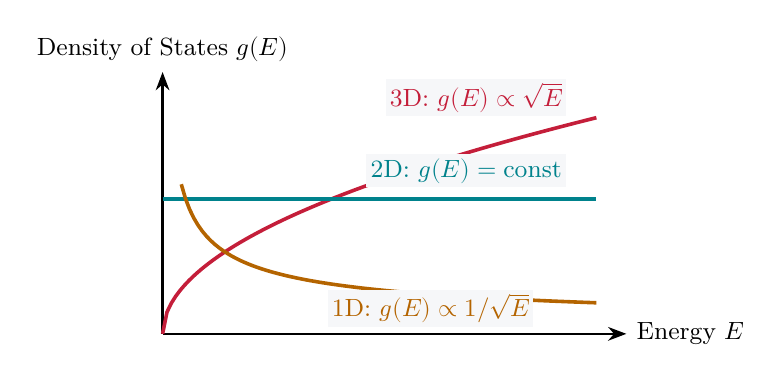
\begin{tikzpicture}[scale=0.95]
  % Axes
  \draw[-Stealth, thick] (0,0) -- (6.2,0) node[right] {\small Energy $E$};
  \draw[-Stealth, thick] (0,0) -- (0,3.5) node[above] {\small Density of States $g(E)$};

  % 3D Curve (Square root)
  \draw[myred, line width=1.3pt, domain=0:5.8, samples=100] plot (\x, {1.2*sqrt(\x)});
  \node[myred, fill=mygray, inner sep=1.5pt, anchor=south east] at (5.4, 2.9) {\small 3D: $g(E) \propto \sqrt{E}$};

  % 2D Curve (Constant)
  \draw[myteal, line width=1.3pt, domain=0:5.8] plot (\x, {1.8});
  \node[myteal, fill=mygray, inner sep=1.5pt, anchor=south east] at (5.4, 1.95) {\small 2D: $g(E) = \text{const}$};

  % 1D Curve (1/sqrt)
  \draw[myamber, line width=1.3pt, domain=0.25:5.8, samples=100] plot (\x, {1.0/sqrt(\x)});
  \node[myamber, fill=mygray, inner sep=1.5pt, anchor=north west] at (2.2, 0.6) {\small 1D: $g(E) \propto 1/\sqrt{E}$};
\end{tikzpicture}
\end{tcolorbox}

% =============================================================================
% SECTION 3: CLASSICAL AND QUANTUM STATISTICS
% =============================================================================
\section{Maxwell-Boltzmann, Bose-Einstein, and Fermi-Dirac Statistics}

\subsection{Qualitative and Quantitative Treatment}

Depending on particle distinguishability, quantum spin, and wave function symmetry:

\begin{tcolorbox}[formulabox, title={\textbf{Three Distribution Functions}}]
\begin{itemize}[leftmargin=*, itemsep=3pt]
  \item \textbf{Maxwell-Boltzmann (MB):} Classical, distinguishable particles, no spin restriction:
  \begin{equation}
  f_{\text{MB}}(E) = A e^{-E / k_B T}
  \end{equation}
  \item \textbf{Bose-Einstein (BE):} Quantum, indistinguishable particles with integer spin ($s=0, 1, 2, \ldots$, Bosons):
  \begin{equation}
  f_{\text{BE}}(E) = \frac{1}{e^{(E-\mu)/k_B T} - 1}
  \end{equation}
  \item \textbf{Fermi-Dirac (FD):} Quantum, indistinguishable particles with half-integer spin ($s=1/2, 3/2, \ldots$, Fermions), obeys Pauli Exclusion Principle:
  \begin{equation}
  f_{\text{FD}}(E) = \frac{1}{e^{(E-E_F)/k_B T} + 1}
  \end{equation}
\end{itemize}
\end{tcolorbox}

\textbf{Comprehensive 8-Criterion Comparison Table:}\par\vspace{6pt}\noindent
\begin{tabularx}{\linewidth}{|B{2.8cm}|Y|Y|Y|}
\hline
\textbf{Feature} & \textbf{Maxwell-Boltzmann} & \textbf{Bose-Einstein} & \textbf{Fermi-Dirac} \\
\hline
\textbf{Particle Nature} & Classical, Distinguishable. & Quantum, Indistinguishable. & Quantum, Indistinguishable. \\
\hline
\textbf{Spin} & Any spin (Spin ignored). & Integral spin ($0, 1\hbar, 2\hbar$). & Half-integral spin ($\frac{1}{2}\hbar, \frac{3}{2}\hbar$). \\
\hline
\textbf{Pauli Principle} & Does not apply. & Does not apply. & Strictly obeys Pauli principle. \\
\hline
\textbf{Occupancy/Cell} & Unlimited ($0, 1, 2, \ldots, \infty$). & Unlimited ($0, 1, 2, \ldots, \infty$). & At most one particle ($0$ or $1$). \\
\hline
\textbf{Wave Function} & No wave function overlap. & Symmetric under particle exchange. & Anti-symmetric under particle exchange. \\
\hline
\textbf{Ground State} & All particles rest at $E=0$ as $T \to 0$. & Bose-Einstein Condensation at $T < T_c$. & Occupies up to Fermi level $E_F$ at $T=0\text{ K}$. \\
\hline
\textbf{Physical Examples} & Ideal gas molecules ($\text{He}, \text{Ar}$). & Photons, Phonons, $\alpha$-particles, $^4\text{He}$. & Free electrons, Protons, Neutrons, $^3\text{He}$. \\
\hline
\end{tabularx}

% =============================================================================
% SECTION 4: FERMI ENERGY & BEC
% =============================================================================
\section{Fermi Energy and Bose-Einstein Condensation}

\subsection{Fermi Energy and Fermi-Dirac Function at T = 0 K}

The \textbf{Fermi Energy ($E_F$)} is the highest filled energy level in a fermion system at absolute zero temperature ($T = 0\text{ K}$).

At $T = 0\text{ K}$:
\begin{equation}
f_{\text{FD}}(E) = 
\begin{cases} 
1 & \text{if } E < E_F \\ 
0 & \text{if } E > E_F 
\end{cases}
\end{equation}
Total number of free electrons $N = \int_0^{E_{F0}} g_e(E) dE = \int_0^{E_{F0}} \frac{8\pi V (2m)^{3/2}}{h^3} E^{1/2} dE = \frac{16\pi V (2m)^{3/2}}{3 h^3} E_{F0}^{3/2}$.

\begin{tcolorbox}[formulabox, title={\textbf{Fermi Energy and Average Energy at T = 0 K}}]
Solving for $E_{F0}$ in terms of electron density $n = N/V$:
\begin{equation}
E_{F0} = \frac{h^2}{8m} \left( \frac{3 N}{\pi V} \right)^{2/3} = \frac{\hbar^2}{2m} (3\pi^2 n)^{2/3}
\end{equation}
The total kinetic energy of $N$ electrons at $T = 0\text{ K}$ is $E_{\text{total}} = \int_0^{E_{F0}} E \, g(E) dE = \frac{3}{5} N E_{F0}$.
Average energy per electron at $T = 0\text{ K}$:
\begin{equation}
\langle E \rangle = \frac{3}{5} E_{F0}
\end{equation}
\end{tcolorbox}

\begin{tcolorbox}[examplebox, title={\textbf{Solved Problem 2: Fermi Energy of Copper}}]
\textbf{Problem:} Copper has free electron density $n = 8.49 \times 10^{28}\text{ m}^{-3}$. Calculate: (a) Fermi energy $E_F$ in eV, (b) Fermi velocity $v_F$.

\textbf{Solution:}\par\noindent
\begin{enumerate}[leftmargin=*, itemsep=2pt]
  \item Fermi energy $E_{F0} = \frac{\hbar^2}{2m} (3\pi^2 n)^{2/3}$:
   $3\pi^2 n = 3 \pi^2 (8.49 \times 10^{28}) = 2.514 \times 10^{29}\text{ m}^{-3}$.
   $(3\pi^2 n)^{2/3} = 3.983 \times 10^{19}\text{ m}^{-2}$.
   \begin{equation}
   E_{F0} = \frac{(1.054 \times 10^{-34})^2}{2 \times (9.11 \times 10^{-31})} \times 3.983 \times 10^{19} = 2.428 \times 10^{-18}\text{ J} = \mathbf{7.04\text{ eV}}
   \end{equation}
  \item Fermi velocity $v_F = \sqrt{\frac{2 E_F}{m}} = \sqrt{\frac{2 \times 2.428 \times 10^{-18}}{9.11 \times 10^{-31}}} = \mathbf{1.57 \times 10^6\text{ m/s}}$.
\end{enumerate}
\end{tcolorbox}

\subsection{Bose-Einstein Condensation (BEC)}

At extremely low temperatures below a critical transition temperature $T_c$, a substantial fraction of bosons collapse into the lowest quantum ground state ($E=0$), forming a macroscopic quantum state known as \textbf{Bose-Einstein Condensate}.

\begin{tcolorbox}[formulabox, title={\textbf{Critical Temperature and Ground State Fraction}}]
Critical BEC transition temperature $T_c$:
\begin{equation}
T_c = \frac{h^2}{2\pi m k_B} \left( \frac{N}{2.612 \, V} \right)^{2/3}
\end{equation}
Fraction of bosons in ground state for $T < T_c$:
\begin{equation}
\frac{N_0}{N} = 1 - \left(\frac{T}{T_c}\right)^{3/2}
\end{equation}
\end{tcolorbox}

% =============================================================================
% QUICK REVISION PAGE
% =============================================================================
\newpage
\begin{center}
  {\large\bfseries\color{myred} Quick Revision --- Module 5}\\[3pt]
  {\small\color{mydark} Statistical Mechanics $|$ BS-PH101}
\end{center}
\noindent{\color{myred}\rule{\linewidth}{1.2pt}}
\vspace{4pt}

\begin{tcolorbox}[formulabox, title={\textbf{Key Formulas and Metrics at a Glance}}]
\renewcommand{\arraystretch}{1.35}
\begin{tabularx}{\linewidth}{B{5.0cm} X}
Boltzmann Entropy Relation & $S = k_B \ln W \quad (W = \text{thermodynamic probability})$ \\[4pt]
Elementary Phase Cell & $d\Omega = h^3 \quad (\text{quantum phase space volume})$ \\[4pt]
3D Density of States & $g_e(E)dE = \frac{8\pi V (2m)^{3/2}}{h^3} E^{1/2} dE$ \\[4pt]
MB Distribution Function & $f_{\text{MB}}(E) = A e^{-E / k_B T}$ \\[4pt]
BE Distribution Function & $f_{\text{BE}}(E) = \frac{1}{e^{(E-\mu)/k_B T} - 1} \quad (\text{Bosons, Integer spin})$ \\[4pt]
FD Distribution Function & $f_{\text{FD}}(E) = \frac{1}{e^{(E-E_F)/k_B T} + 1} \quad (\text{Fermions, Half-spin})$ \\[4pt]
Fermi Energy ($T=0\text{ K}$) & $E_{F0} = \frac{h^2}{8m}\left(\frac{3N}{\pi V}\right)^{2/3} = \frac{\hbar^2}{2m}(3\pi^2 n)^{2/3}$ \\[4pt]
Average Fermi Energy & $\langle E \rangle = \frac{3}{5} E_{F0} \quad (\text{at } T=0\text{ K})$ \\[4pt]
BEC Transition Temp. & $T_c = \frac{h^2}{2\pi m k_B} \left(\frac{N}{2.612 \, V}\right)^{2/3}$ \\[4pt]
BEC Condensate Fraction & $\frac{N_0}{N} = 1 - \left(\frac{T}{T_c}\right)^{3/2} \quad (\text{for } T < T_c)$ \\[4pt]
\end{tabularx}
\end{tcolorbox}

\begin{tcolorbox}[defbox, title={\textbf{One-Line Definitions}}]
\begin{itemize}[leftmargin=*, itemsep=2pt]
  \item \textbf{Microstate:} A specific detailed microscopic specification of position and momentum coordinates for all particles in a system.
  \item \textbf{Ensemble:} A large virtual collection of independent, macroscopically identical systems in different microstates.
  \item \textbf{Fermi Energy ($E_F$):} The maximum energy state occupied by free electrons at absolute zero temperature ($T=0\text{ K}$).
  \item \textbf{Boson:} A particle with integral quantum spin ($0, 1\hbar, 2\hbar$) obeying Bose-Einstein statistics and symmetric under particle exchange.
  \item \textbf{Bose-Einstein Condensation:} A phase transition where a macroscopic number of bosons collapse into the single lowest energy ground state at $T < T_c$.
\end{itemize}
\end{tcolorbox}

\begin{tcolorbox}[exambox, title={\textbf{Frequently Asked / Viva Questions}}]
\begin{enumerate}[topsep=0pt, label=\textbf{Q\arabic*.}, itemsep=5pt]
  \item \Q{What is the difference between a macrostate and a microstate?}
  A macrostate specifies overall macroscopic variables $(N,V,E)$; a microstate specifies exact microscopic position and momentum coordinates $(\vec{r}_i, \vec{p}_i)$ of every particle.

  \item \Q{What is phase space and what is its minimum volume in quantum mechanics?}
  Phase space is a $6N$-dimensional space combining 3 position and 3 momentum axes per particle. Its minimum volume cell in quantum mechanics is $h^3$.

  \item \Q{Distinguish between Microcanonical, Canonical, and Grand Canonical ensembles.}
  Microcanonical keeps $(N,V,E)$ fixed; Canonical keeps $(N,V,T)$ fixed (heat exchange allowed); Grand Canonical keeps $(\mu,V,T)$ fixed (heat and particle exchange allowed).

  \item \Q{State the basic difference between Bosons and Fermions.}
  Bosons have integral spin ($0, 1\hbar$), symmetric wavefunctions, and do not obey Pauli principle. Fermions have half-integral spin ($\frac{1}{2}\hbar$), anti-symmetric wavefunctions, and strictly obey Pauli principle.

  \item \Q{Why does density of states in 3D vary as $\sqrt{E}$?}
  Because the momentum sphere volume $V_p \propto p^3 \propto E^{3/2}$. Taking the derivative $g(E) = dN/dE$ gives $g(E) \propto E^{1/2} = \sqrt{E}$.

  \item \Q{Draw Fermi-Dirac distribution curve at $T = 0\text{ K}$ and $T > 0\text{ K}$.}
  At $T = 0\text{ K}$, $f(E)$ is a step function ($f=1$ for $E < E_F$, $f=0$ for $E > E_F$). At $T > 0\text{ K}$, thermal agitation creates a symmetric tail around $E_F$ where $f(E_F) = 1/2$.

  \item \Q{What is the physical meaning of Fermi energy?}
  Fermi energy represents the highest energy level occupied by free conduction electrons in a metal at absolute zero temperature ($T=0\text{ K}$).

  \item \Q{Calculate the average energy of an electron gas at $T = 0\text{ K}$ in terms of $E_F$.}
  $\langle E \rangle = \frac{\int_0^{E_F} E \cdot E^{1/2} dE}{\int_0^{E_F} E^{1/2} dE} = \frac{\frac{2}{5} E_F^{5/2}}{\frac{2}{3} E_F^{3/2}} = \frac{3}{5} E_{F0}$.

  \item \Q{Under what conditions do BE and FD statistics reduce to MB statistics?}
  At high temperatures ($T \to \infty$) and low particle densities ($n \to 0$), when $e^{(E-\mu)/k_B T} \gg 1$, both BE and FD distributions reduce to classical MB distribution $f(E) \approx e^{-(E-\mu)/k_B T}$.

  \item \Q{What is Bose-Einstein Condensation (BEC)?}
  BEC is a low-temperature phenomenon where a macroscopic fraction of bosons condense into the single zero-momentum ground state at $T < T_c$.

  \item \Q{Why can photons undergo BEC without fixing total particle number $N$?}
  Photons have chemical potential $\mu = 0$ because photon number is not conserved (photons are freely created/absorbed by cavity walls).

  \item \Q{Why do electrons in a metal not contribute significantly to heat capacity at room temperature?}
  Because Pauli exclusion principle restricts thermal excitation ($k_B T$) to only a small fraction ($\sim k_B T / E_F \approx 1\%$) of electrons near the Fermi level $E_F$.
\end{enumerate}
\end{tcolorbox}

\begin{tcolorbox}[tikzbox, title={Summary Comparison of Quantum Statistics}]
\centering
\begin{tabularx}{\linewidth}{|B{3.2cm}|Y|Y|Y|}
\hline
\textbf{Property} & \textbf{Maxwell-Boltzmann} & \textbf{Bose-Einstein} & \textbf{Fermi-Dirac} \\
\hline
\textbf{Distribution Eq.} & $f(E) \propto e^{-E/k_B T}$ & $f(E) = \frac{1}{e^{(E-\mu)/k_B T} - 1}$ & $f(E) = \frac{1}{e^{(E-E_F)/k_B T} + 1}$ \\
\hline
\textbf{Ground State Occupancy} & Non-zero classical energy. & Condensate ($N_0$ particles at $E=0$). & Filled Fermi sphere up to $E_F$. \\
\hline
\textbf{Wave Symmetry} & Distinguishable (No symmetry). & Symmetric under exchange. & Anti-symmetric under exchange. \\
\hline
\end{tabularx}
\end{tcolorbox}

\end{document}
